\documentclass[compsoc,conference,a4paper,10pt,times]{IEEEtran}
% \IEEEoverridecommandlockouts
% The preceding line is only needed to identify funding in the first footnote. If that is unneeded, please comment it out.   
\usepackage{cite}
\usepackage{amsmath,amssymb,amsfonts}
\usepackage{algorithmic}
\usepackage{graphicx}
\usepackage{textcomp}
\usepackage{bmpsize}
\usepackage{xcolor}
\usepackage{lipsum}
\usepackage[colorlinks=true,urlcolor=black]{hyperref}
\def\BibTeX{{\rm B\kern-.05em{\sc i\kern-.025em b}\kern-.08em
    T\kern-.1667em\lower.7ex\hbox{E}\kern-.125emX}}

\usepackage{minted}    

\usepackage[inline]{enumitem}
\usepackage[all,cmtip]{xy}
% New commands
\newtheorem{theorem}{Theorem}[section]
\newtheorem{corollary}{Corollary}[theorem]
\newtheorem{lemma}[theorem]{Lemma}
\newtheorem{defin}[theorem]{Definition}
\newtheorem{example}[theorem]{Example}

% take this out for final version
\pagestyle{plain}

\usepackage{graphicx}
% \graphicspath{ {/Users/bahman.sistany/bahman_mac/imp} }

\begin{document}

\title{Towards Formal Verification of Program Obfuscation}

\author{\IEEEauthorblockN{Weiyun Lu\IEEEauthorrefmark{1},
    Bahman Sistany\IEEEauthorrefmark{2},
    Amy Felty\IEEEauthorrefmark{1}\IEEEauthorrefmark{3},
    Philip Scott\IEEEauthorrefmark{3}\IEEEauthorrefmark{1}}
  \IEEEauthorblockA{\IEEEauthorrefmark{1}School of Electrical
    Engineering and Computer Science, University of Ottawa, Canada\\
    Email: \{wlu058,afelty,philip.scott\}@uottawa.ca}
  \IEEEauthorblockA{\IEEEauthorrefmark{2}Cloakware Research
    Irdeto Canada, Ottawa, Canada\\
    Email: bahman.sistany@irdeto.com}
  \IEEEauthorblockA{\IEEEauthorrefmark{3}Department of Mathematics and
    Statistics, University of Ottawa, Canada}}

%\author{\IEEEauthorblockN{Weiyun Lu}
%\IEEEauthorblockA{\textit{School of Electrical Engineering and Computer Science} \\
%\textit{University of Ottawa}\\
%Ottawa, Canada \\
%WLU058@uottawa.ca}
%\and
%\IEEEauthorblockN{Bahman Sistany}
%\IEEEauthorblockA{\textit{Cloakware Research} \\
%\textit{Irdeto Canada}\\
%Ottawa, Canada \\
%bahman.sistany@irdeto.com}
%\and
%\IEEEauthorblockN{Amy Felty}
%\IEEEauthorblockA{\textit{School of Electrical Engineering and Computer Science} \\
%\textit{University of Ottawa}\\
%Ottawa, Canada \\
%afelty@uottawa.ca}
%\and
%\IEEEauthorblockN{Philip Scott}
%\IEEEauthorblockA{\textit{School of Electrical Engineering and Computer Science} \\
%\textit{University of Ottawa}\\
%Ottawa, Canada \\
%philip.scott@uottawa.ca}
%}

\maketitle

\begin{abstract}

%\par How can one perform code transformations such as obfuscating transformations or optimizing transformations on code that is assumed to be correct with respect to certain specified behaviour? Will the transformed code preserve the specified behaviour as one expects? 

%\par To achieve the highest levels of assurance that the transformations have maintained correctness of the code, is to prove the two versions of the program (before and after the transformation) are equivalent, but proving program behaviour equivalency in general is hard. Forgoing general program behaviour equivalency, what if we directly try to show validity of originally specified behaviour on the transformed program? 

%\par In this research, we lay the foundation to study and reason about code obfuscating transformations and show how the preservation of certain behaviours may be ``certified''. To this end, we apply techniques of formal specification and verification, by using the Coq Proof Assistant and IMP (a simple imperative language within it), to formulate what it means for a program's semantics to be preserved by an obfuscating transformation, and give formal machine-checked proofs that these behaviours or proerties hold. 

%\par We describe our work on opaque predicates, a simple control flow obfuscation, and elements of control flow flattening transformation, a more complex control flow obfuscation.  Along the way, we employ Hoare logic as our foundational specification language, as well as augment the IMP language with Switch statements.  We also define a lower-level flowchart language to wrap around IMP for modelling certain flattening transformations, treating blocks of codes as objects in their own right.

Code obfuscation involves transforming a program to a new version that performs the same computation but hides the functionality of the original code.  An important property of such a transformation is that it preserves the behavior of the original program.
In this paper, we lay the foundation for studying and reasoning about code obfuscating transformations, and show how the preservation of certain behaviours may be formally verified. To this end, we apply techniques of formal specification and verification using the Coq Proof Assistant.  We use and extend an existing encoding of a simple imperative language in Coq along with an encoding of Hoare logic for reasoning about this language.  We formulate what it means for a program's semantics to be preserved by an obfuscating transformation, and give formal machine-checked proofs that these behaviours or properties hold. We also define a lower-level block-structured language which is ``wrapped around'' our imperative language, allowing us to model certain flattening transformations and treat blocks of codes as objects in their own right.
\end{abstract}

\begin{IEEEkeywords}
obfuscation, verification, security, correctness, Coq, proof
\end{IEEEkeywords}

\section{Introduction}
We expect our software systems to function correctly. By ``correctly'', we mean that a system will behave according to explicit and/or implicit expectations, i.e., its written and/or unwritten specifications. Typically, extensive testing is done to increase the confidence in the correct functionality of a piece of software.

%but alas testing is known to be based on inductive reasoning where more tests passing can only increase the likelihood of correctness, so positive testing results are not a proof of correctness. 
%I don't think it is correct to say inductive reasoning.  Most of our reasoning is Coq is by induction.  So, I changed the wording.
The more testing that is done, the more confidence one has of the likelihood of correctness, but positive testing results are not a proof of correctness.
In systems where more assurance of correctness is required, various types of deductive reasoning are often used, where formal verification methods based on theoretical foundations rooted in logic are employed. This is the approach that we adopt here.  It is important to note that formal verification transfers the problem of confidence in program correctness to the problem of confidence in specification correctness.  Thus, it is not a silver bullet; however, since specifications are often smaller and less complex to express, we are able to successfully reduce the trusted computing base (TCB) and increase our chances of achieving correctness.

%Formal verification based methods, used to show a (software) system behaves as its specification says, typically employ a specification language based on the familiar ``assertions''. A specification is typically expressed in some variation of first order logic and the verification system will deductively try to prove the assertions correct or signal that they don't hold. This is a rather elaborate process where assertions (general propositional statements about program fragments that are expected to hold) are used to generate verification conditions (VC), logic formulas, that are then fed into a satisfiability modulo theories (SMT) solver, either behind the scenes in a verification backend or in more visible to the verification expert. VC generation for program verification goes back to at least Hoare's triples, Eiffel style contracts and proof-carrying-code (PCC) of Necula\cite{b7}.
A common approach to formal verification used to show a (software) system behaves according to its specification is to employ a specification language based on the familiar use of \emph{assertions} \cite{Floyd,Hoare}. A specification (in the form of statements about program fragments that are expected to hold) is typically expressed in some variation of first-order logic, and the verification system will try to either prove the assertions correct or signal that they don't hold. This can be a rather elaborate process.  For example, assertions can be used to generate logical formulas called \emph{verification conditions} (VCs), which are either fed into a \emph{satisfiability modulo theories} (SMT) \cite{ge2007solving} solver behind the scenes in a verification backend, or are presented in a more visible manner to a verification expert who will manually discharge them. VC generation for program verification goes back to at least Hoare logic \cite{Hoare}, Eiffel style contracts \cite{Eiffel}, and proof-carrying-code (PCC) \cite{b7}.

In this paper, we use a formal verification approach to the task of program transformations.
In particular, the question we address here is:
how can one perform obfuscating or optimizing transformations on code that is assumed to be correct with respect to certain specified behaviour (expressed in some assertion language) while preserving the correctness of the specified behaviour?

%To achieve the highest levels of assurance that the transformations have maintained correctness of the code, is to prove the two versions of the program (before and after the transformation) is equivalent. Proving equivalency is doable in certain cases but in general is still extremely hard to do for general programs. Despite the difficulty, there are now formally verified compilers such as CompCert. However, the problem with verifying realistic systems such as a compiler is scale. CompCert verification of semantic equivalence between C and generated assembly took several man years to complete. The cost of using formal verification for mere mortals (on realistic systems) is still high. 
To achieve the highest level of assurance that a transformation has maintained correctness of the code, one should prove that the two versions of the program (before and after the transformation) are equivalent. Although there exist large-scale verification results such as the formally verified compiler CompCert \cite{CompCert}, in general scaling up verification efforts to realistic systems is extremely hard. CompCert involved the verification of a semantic equivalence between C and a generated assembly language, and took several man-years to complete. 

%
Equivalence between two versions of a program certainly implies the correctness of any program properties of interest proved for one version applies to the other.  Alternatively, what if we limit ourselves to only proving properties of interest in the ``before'' version of a program, and show that these properties are maintained in the ``after'' version of the program after a particular transformation is applied? 
%
%Certain simple transformations simply don't invalidate expressed properties about the ``before'' version versus the ``after'' version. Below the program snippet in listing [\ref{lst:before}] asserts that $y > 2$ which we can verify visually to be true. In the snippet in listing [\ref{lst:after}] we use a simple obfuscating transformation called variable splitting where we have split the variable $x$ into two other variables $x1$ and $x2$ and we see that (visually) the assertion $y > 2$ still holds.
Here, our focus is on certain simple transformations that don't invalidate properties about the ``before'' version versus the ``after'' version.  For example, consider the program snippet in Listing \ref{lst:before}, which asserts that \texttt{(y > 2)} and is easily verified visually. The snippet in Listing \ref{lst:after} illustrates a simple obfuscating transformation called \emph{variable splitting}, where we have split the variable \texttt{x} into two  variables \texttt{x1} and \texttt{x2}, and it is clear (visually) that the assertion \texttt{(y > 2)} still holds.


\begin{listing}
\caption{Original Code}
\label{lst:before}
\begin{minted}
[
frame=single,
framesep=2mm,
baselinestretch=1.2,
fontsize=\footnotesize
] {c}
x = 2; y = 5;
y = x + y;
assert(y > 2);
\end{minted}
\end{listing}

\begin{listing}
\caption{Obfuscated Code}
\label{lst:after}
\begin{minted}
[
frame=single,
framesep=2mm,
baselinestretch=1.2,
fontsize=\footnotesize
] {c}
x1 = 1; x2 = 1; y = 5;
y = x1 + y; y = x2 + y;
assert(y > 2);
\end{minted}
\end{listing}

In general, though, most transformations, whether optimizations or obfuscations,
%but especially obfuscations which are the focus of this paper, 
invalidate assertions that hold true about the ``before'' version. Obfuscation is particularly troublesome, because its main goal is to hide the functionality of the code from prying eyes while maintaining the functionality of the ``before'' program. More formally, according to Barak et al. as cited in \cite{BanescuCGNP16}, obfuscators are programs that transform an input program (e.g. similar to a compiler) into an output program such that the output program satisfies the following three properties:
\begin{enumerate}
   \item it is semantically equivalent to the input program (\emph{functionality property}); \label{itm:firstproperty}
   \item it is at most polynomially bigger or slower than the input program (\emph{slowdown} property); and \label{itm:secondproperty}
   \item it is as ``hard to analyze and de-obfuscate'' as a blackbox version of the program (\emph{virtual black-box property}). \label{itm:thirdproperty}
\end{enumerate}
%``Prying eyes'' could as easily be the same as some kind of static analysis tool where an attacker is trying to determine certain facts about the code and obfuscation is trying to make this difficult. The program in listing [\ref{lst:beforeopaque}] is correct with respect to the assertion that is expressed (e.g. $z == 30$) as is evident by simple inspection of the code. The program snippet in listing [\ref{lst:afteropaque}] is the ``after'' program where a non-linear opaque predicate transformation has been applied to hide the fact that at program's end, value of $z$ is in fact 30. We can see that the transformation makes it a bit harder to see that the assertion still holds but knowing the fact that $\forall x \in \mathbb{Z}, ((x^2 + x)\bmod 2) == 0$ , we can deduce that the assertion does hold and the value of $z$ is in fact still 30. 
``Prying eyes'' could, for example, be some kind of static analysis tool where an attacker is trying to determine certain facts about the code, and obfuscation is trying to make this difficult. The program in Listing \ref{lst:beforeopaque} is correct with respect to the assertion that is expressed (e.g. \texttt{z == 30}) as is evident by simple inspection of the code. The program snippet in Listing \ref{lst:afteropaque} is the ``after'' program where a non-linear \emph{opaque predicate transformation} (see Section~\ref{sec:opaque}) has been applied to hide the fact that at program's end, the value of \texttt{z} is in fact \texttt{30}. In this case, it follows from the fact that $\forall x \in \mathbb{Z}, ((x^2 + x)\bmod 2) = 0$. 

%This paper describes steps towards implementing a framework in the Coq Proof Assistant and based on IMP\cite{SFV2}, a simple imperative language to study obfuscating transformations, their impact on programs and how specified behaviour may be preserved beyond the transformations. A number of initial goals and principles drove the direction of this research: 
This paper describes steps towards implementing a framework in the Coq Proof Assistant \cite{Coq} for a simple imperative language that allows us to study obfuscating transformations, their impact on programs, and how specified behaviour may be preserved beyond the transformations. Our starting point is the IMP language from \cite{SFV2}, which includes an encoding in Coq of a familiar small imperative language along with its formalized semantics.
A number of initial goals and principles drove the direction of this research: 
%\begin{enumerate*}
 % \item We don't want to reinvent the wheel, which is why we start with IMP: start out with IMP a familiar small imperative language implemented in Coq and use its accompanying formalized semantics in \cite{SFV2}.
 % \item Accessibility to as wide an audience as possible: an obvious option was to use CompCert and Clight as \cite{Blazy2} has done. We would have started with lots of proofs and formalisms for free (already done by the CompCert team) however the significant learning curve associated with learning CompCert infrastructure seemed prohibitive. We deemed IMP and the Coq infrastructure much more accessible.\label{goal2}
 % \item Extendibility of the framework: Following the lead of \cite{SFV2} where a number of extensions to IMP are easily added and studied, we wanted the ability to build our obfuscation infrastructure incrementally on top of IMP.\label{goal3}
 % \end{enumerate*} 
 \begin{enumerate}
  \item We don't want to reinvent the wheel, which is why we start with IMP.
  \item We want to assure accessibility to as wide an audience as possible. For this reason, we choose IMP over CompCert and Clight, which are used in \cite{Blazy2}.  On the one hand, building on CompCert would have given us lots of proofs and formalisms for free; however, the significant learning curve associated with this infrastructure seemed prohibitive, and thus much less accessible.\label{goal2}
  \item We want the framework to be extendable.  Following the lead of \cite{SFV2}, where a number of extensions to IMP are easily added and studied, we wanted the ability to build our obfuscation infrastructure incrementally on top of IMP.\label{goal3}
  \end{enumerate}

 \begin{listing}
\caption{Original Code}
\label{lst:beforeopaque}
\begin{minted}
[
frame=single,
framesep=2mm,
baselinestretch=1.2,
fontsize=\footnotesize
] {c}
int main (int argc, char *argv[])
{
  unsigned int x = 10;
  unsigned int y = 20;
  unsigned int z = 0;

  z = x + y;
  assert(z == 30);
  return 0;
}
\end{minted}
\end{listing}

\begin{listing}
\caption{Obfuscated Code}
\label{lst:afteropaque}
\begin{minted}
[
frame=single,
framesep=2mm,
baselinestretch=1.2,
fontsize=\footnotesize
] {c}
int main (int argc, char *argv[])
{
  unsigned int x = 10;
  unsigned int y = 20;
  unsigned int z = 0;

  unsigned int a = ((unsigned int)argc);
  unsigned int w = a * a;

  w = a + w;
  w = w % 2;
  if (w == 0)
  {
    z = x + y;
  }
  else
  {
    z = y - x;
  }
  assert(z == 30);
  return 0;
}
\end{minted}
\end{listing}
 
Keeping these research goals in mind the contributions of this paper are the following:
\begin{itemize}
    \item \label{itm:1} We consider different formulations of what it means for a transformation to be semantics-preserving: we cover \emph{command equivalence} in Sections \ref{commequiv} and \ref{naive} as well as \emph{Hoare logic equivalence} in Section \ref{hoarequiv}. By command equivalence, we mean that if the two programs start out in the same state, then the state resulting after execution of each program is exactly the same.  By state, we mean variable names and their values; these values can change during execution, but at the end, all variable values must have changed in exactly the same way.  
    %This is the notion of equivalence mentioned above. 
    Hoare logic equivalence is a weaker notion that is enough for most code obfuscation transformations. It allows an obfuscated program to use and modify variables that don't occur in the assertion.  Only the values of variables that occur in the assertion are required to have the same values at the end of execution.  Using Hoare logic equivalence in this particular setting is a novel approach, helping us establish a central strategy to ``Formal Verification of Program Obfuscation'': our obfuscated programs will be ``decorated''  \`a la  Pierce \cite{SFV2} with additional assertions whose proofs will also be provided. The additional assertions that our obfuscators will provide will be needed to show the original desired behaviour still holds after an obfuscation.
    %\footnote{Bahman and Amy: find a good place to cover this proposal and if so update the reference to \ref{hoarequiv} above.}
    
    
    \item We give motivations and a top-level explanations for all of the transformations and one of the proofs (the main one in Section~\ref{sec:flattening}).  Proofs in Coq are done by giving step-by-step commands called \emph{tactics}, which break the goal (the statement to be proven) into subgoals until each branch of the proof is completed.  (We don't discuss tactics, but
    %\footnote{AF: We agreed to remove this paragraph.  I am leaving it here for now until we figure out where to refer to Wei's thesis, and maybe include a discussion about this at that point.}
    refer the reader to \cite{Weiyun} for a more detailed treatment of both the proofs and tactics.) 
    %To the best of our knowledge, the existing literature does not provide this level of detail, which here provides an accessible explanation of not just obfuscation techniques, but also in tandem with its formalization and verification inside Coq. This follows from research goal \ref{goal2} above.%\footnote{Phil asks Why?}\label{itm:2}
    To the best of our knowledge, the existing literature does not provide this level of detail. We provide not only an accessible explanation of obfuscation techniques but also their formalization and verification inside Coq. This follows along the lines of research goal \ref{goal2}. 
 
    %\item We begin with a minimal imperative programming language inside Coq for reasoning about programs and their transformations, and then augment it as needed for control flow flattening algorithms, first by augmenting its syntax and semantics with switch statements, and then by defining a lower-level flowchart language that wraps around blocks of code in order to model real-world intermediate languages used in obfuscation tools. This follows our research goals \ref{goal2} and \ref{goal3}. \label{itm:3}
   \item We begin with a minimal version of IMP and augment it as needed for \emph{control flow flattening algorithms} (see Section~\ref{sec:flattening}),
   %\footnote{AF: Like ``opaque predicate transformation'', I put this in italics and I think it needs a forward reference.} 
   first by augmenting its syntax and semantics with switch statements, and then by defining a lower-level block-structured language that wraps around blocks of code in order to model real-world intermediate languages used in obfuscation tools. This contributes to research goals \ref{goal2} and \ref{goal3}. \label{itm:3}
\end{itemize}

This project, and in particular, the formalization in Coq, was motivated by the Cloakware obfuscation tool produced at Irdeto, and the interest in showing the correctness of some of its core functionality in safety critical environments.\footnote{Much of it was carried out during the first author's co-op term at Irdeto under the supervision of the second author. The first author further developed it in his Master's thesis \cite{Weiyun}; all lemmas and theorems referred to in this paper are formally proved in Coq.} For details of the Coq code and fuller explanations of the proofs, the reader is referred to \cite{WeiRepo} and \cite{Weiyun}, respectively.
%\footnote{Bahman: just marking references to Wei's work. At the end, some may be redundant and/or out of place.}\footnote{AF: I moved this text up from Section 2 to Section 1, and I think we can remove many/most of the other references to the Coq code and the proofs (which I have done). I think this addresses Phil's comments (top of page 1 and the bottom of page 2 on his annotated pdf, and comment 2 in his email).}


%\section{Background --- formal verification}\label{two}
%In this chapter we provide necessary background information used for formal verification --- namely, the Coq proof assistant, the simple imperative language IMP defined inside Coq, and Hoare logic for reasoning about pre- and post-conditions of programs.
%\subsection{The Coq proof assistant}

%Coq \cite{Coq} is a formal proof management system, an implementation of the \emph{Calculus of (co)inductive constructions}, which provides a formal language in which one can write mathematical definitions, algorithms and theorems, and an environment for the development of machine-checked proofs.  It is implemented (mostly) in OCaml\footnote{See \href{https://www.ocaml.org}{https://www.ocaml.org}.} and (a little bit of) C.

\section{The IMP Language and Hoare Logic}
We now give the necessary definitions from Software
Foundations \cite{SFV2} needed to understand our formalization in the
sections that follow.  Along the way, we describe the features of Coq
that we use.  
%This project, and in particular, the formalization in Coq, was motivated by the Cloakware obfuscation tool produced at Irdeto, and the interest in showing the correctness of some of its core functionality in safety critical environments.\footnote{Much of it was carried out during the first author's co-op term at Irdeto under the supervision of the second author.}
For more details on IMP, the reader is referred to \cite{SFV2}.
%, while for details of the code in later sections, the reader is referred to our repository \cite{WeiRepo}\footnote{Bahman: just marking references to Wei's work. At the end, some may be redundant and/or out of place}.

%We now give the necessary definitions and theorems from Software Foundations \cite{SFV2}.\footnote{AF: As Wei mentioned, we don't define IMP, but I think we need to in order for the reader to understand the rest of the paper.  We need to define \texttt{com} and \texttt{state} along with all of the notation we use for them (e.g., so that the reader can understand any of the programs like fact\_nonzero).  We need to define the evaluation and the notation used for it (e.g., c / st backslash st').  As well as any other basic definitions and notations used in what is now Section 3.}

\subsection{Syntax and Semantics of IMP}
\label{sec:syntaxsemantics}
Informally, IMP commands are defined by the following BNF grammar:
\texttt{c ::= SKIP | x ::= a | c ;; c | IFB b THEN c ELSE c FI | WHILE b DO c END}.
In~\cite{SFV2}, this grammar is encoded by defining a new type called \texttt{com} and new keywords (called \emph{constructors} in Coq), one for each element of the grammar, and then defining notation that maps this formal definition to the BNF syntax.  For example, the definition of \texttt{com} includes the following case for assignment statements: \texttt{CAss (x : string) (a : aexp)}, which introduces the \texttt{CAss} constructor and specifies its two arguments along with their types.  A variable is represented using the built-in \texttt{string} type in Coq, the arithmetic expression on the right of an assignment command has type \texttt{aexp}, and the notation specifies that Coq terms of the form \texttt{(CAss x a)} will be written \texttt{x := a}.
The definition of \texttt{aexp} in~\cite{SFV2} is defined using the same technique---starting from a BNF grammar, constructors are defined and then notation is given so that the syntax matches the grammar.  We omit its definition as well as the definition of \texttt{bexp} for representing boolean expressions, which appear in \texttt{IFB} and \texttt{WHILE} commands.

To define the operational semantics of IMP, the notion of a state is needed. We introduce a type called \texttt{state} defined to be an abbreviation for the type \texttt{string -> nat}.  Here, \texttt{nat} is Coq's built in type for natural numbers $\mathbb{N}$.  Although, we restrict our formal development to natural numbers, it could be easily extended to other types such as \texttt{int} or \texttt{float}.  An \textit{initial state} in Coq is a function that maps all variables to the default value $0$.  States are modified using an update operator.  For example, the state \verb|s & { X --> 3; Y --> 1}| represents a state in which \texttt{s} is modified so that \texttt{X} has the value \texttt{3} and \texttt{Y} has the value \texttt{1}.  The ``\verb|s &|'' can be omitted if the update is to an initial state.

Evaluation of commands can be viewed as a partial function from a command and a starting state to a new state.  It is encoded as a relation in Coq, and the notation \verb|c / s1 \\ s2| means that starting in state \texttt{s1} and executing \texttt{c} results in a new state \texttt{s2}.  We say that ``\texttt{c} takes \texttt{s1} to \texttt{s2}.''  The definition of this relation relies on two functions.  The first is \texttt{aeval};
the expression \texttt{(aeval s a)} evaluates \texttt{a} (an element of \texttt{aexp}) in a state \texttt{s}, resulting in a natural number. The function \texttt{beval} is similar and maps a \texttt{bexp} to a Coq boolean.  (We omit the details of these definitions.)

%, an interactive textbook on the mathematical foundations of reliable software, which is actually entirely a Coq script.

%\par We use the \emph{IMP} language defined within the Software Foundations Coq files for our code obfuscation formalisms.  IMP, which simply stands for imperative, is a bare-bones simple imperative language, like C stripped of all nonessential features.  This simplicity allows us to focus on the nuts and bolts of formally specifying and proving correct individual obfuscating transformations, emphasizing modularity.

%\par Since IMP is written inside Coq, we can formally reason about not just individual programs, but entire classes of programs, and even the language itself.  We give the definitions, lemmas, and theorems necessary for our work, but will omit many details and proofs (see \cite{Weiyun} for omitted details and \cite{WeiRepo} for the Coq code and further details).  

%\par IMP is built up piece by piece in \cite{SFV2} with multiple iterations (some failed, some tangential) for pedagogical purposes, but we will only present the final form that we end up using.  IMP has the basics of natural number arithmetic, booleans, and commands consisting of assignment, skip, if-then-else, and while-do-end.

\subsection{Command Equivalence Definition}\label{commequiv} 
    For two commands (IMP programs) \texttt{c1} and \texttt{c2} to be command equivalent means that for any pair of states \texttt{st} and \texttt{st'}, \texttt{c1} takes \texttt{st} to \texttt{st'} if and only if \texttt{c2} takes \texttt{st} to \texttt{st'}.  In Coq, \texttt{cequiv}\cite{SFV2}  is defined as a predicate that takes two commands as arguments:
\begin{defin}[Comand equivalence]\label{def:cequiv}
\begin{verbatim}
Definition cequiv (c1 c2 : com) : Prop 
  := forall (st st' : state), 
(c1 / st \\ st') <-> (c2 / st \\ st').
\end{verbatim}
\end{defin}
\texttt{Prop} is the type of logical formulas in Coq, and \texttt{forall} and \texttt{<->} are the notations for universal quantification and logical equivalence, respectively. The corresponding definitions for arithmetic expressions and booleans are also important.
\begin{defin}[Arithmetic/boolean equivalence]
\begin{verbatim}
Definition aequiv (a1 a2 : aexp) : Prop
  := forall s, aeval s a1 = aeval s a2.
Definition bequiv (b1 b2 : bexp) : Prop
  := forall s, beval s b1 = beval s b2.
\end{verbatim}
\end{defin}


\subsection{Hoare Logic}
\emph{Hoare logic} is a way for us to prove that executing a program will result in satisfying certain post-conditions, (possibly) conditional on certain pre-conditions being met.  This involves defining a natural way of writing program specifications, along with a compositional proof technique to prove correctness with respect to them.
\begin{defin}[Hoare triple]
	A \emph{Hoare triple} is a triple consisting of a pre-condition $P$, a program $c$, and a post-condition $Q$, written
    \[
    	(| P |)\ c\ (| Q |),
    \]
    which specifies that whenever $P$ is true before execution, running the program $c$ is guaranteed to make $Q$ true after execution.  
\end{defin}
This informal definition leaves states implicit, but for the formal definition in Coq we will need to take states into account.

\begin{defin}[Assertion]
An \emph{assertion} about a program's state is a function from states to propositions.
\begin{verbatim}   
  Definition Assertion := state -> Prop.
\end{verbatim}
\end{defin}
Informally, for some assertion $P$ and some state $st$, the proposition $(P~st)$ represents the statement that $P$ holds in state $st$.  
As an example, let $st$ be the state where the value of every variable is 0.  Let $P$ be the assertion that $x=0$.  Then $(P~st)$ is the proposition ``$x = 0$ in the state $st$''.  In Coq, Hoare triples have three arguments, a command and two assertions:
\begin{verbatim}
Definition hoare_triple (P:Assertion)
  (c:com) (Q:Assertion) : Prop :=
  forall st st', c / st \\ st'  ->
  P st  -> Q st'.
\end{verbatim}
%Note that in the formal version, states must be explicit.
and expresses that if \texttt{P} holds in state \texttt{st} and \texttt{c} takes \texttt{st} to \texttt{st'}, then \texttt{Q} holds in \texttt{st'}.  We will sometimes use the notation \texttt{\{\{P\}\}c\{\{Q\}\}}  to represent the Coq expression \texttt{(hoare\_triple P c Q)}.

Proving that a Hoare triple holds is a line-by-line affair, starting from the bottom of a program and working upwards.  There is one rule for each kind of IMP command, and the application is mostly mechanical, except for the \texttt{WHILE} statement (see \cite{SFV2}).

\section{Opaque Predicates in IMP/Coq}
\label{sec:opaque}
An \emph{opaque predicate} \cite{CoNa} is a predicate that always evaluates to either \emph{true} or \emph{false} and the truth-value is known to the transformation but hard to deduce by an attacker \cite{Prada}. It could be any boolean expression in a program, but we will only be concerned with those involving arithmetic formulas here. An opaque predicate is used, for example, in an \texttt{IFB} statement, and in the case when it evaluates to \emph{true}, the code under the \emph{false} branch is never evaluated at runtime.  Thus opaque predicates incur no runtime performance penalty.

Of course, the most basic opaque predicates are just the boolean constants \emph{true} and \emph{false} themselves, but these are not very useful in practice because it is immediately obvious what is happening in the program, and neither the simplest of humans nor tools will be fooled. For a more advanced treatment of opaque predicates and how they may be broken see \cite{Prada}.

An \emph{opaque predicate transformation} takes as inputs a program to be obfuscated, \texttt{c1}, an opaque predicate \texttt{P} that takes one argument, and a dummy program \texttt{c2}, and returns the program:
\begin{verbatim}
    IFB (P x) THEN c1 ELSE c2 FI.
\end{verbatim}
It is not known to an attacker, a priori, that \texttt{c2} is a dummy program. In practice, \texttt{c2} should be complicated enough to appear that it could feasibly be intended to be executed. For example, \texttt{c2} is often an actual command/statement randomly chosen to be the dummy program.

In Section \ref{naive}, we describe our initial (straightforward, naive) attempt, in which the transformation introduces new variables (as is standard in writing code in a typical imperative language), assigns them values and then uses them in the opaque predicate.  Using this approach, trying to state a general theorem about command equivalence ends up being problematic.  

We then discuss how this problem spawned two ideas in different directions, which both rectify the issue. First, we keep the above approach to adding variables, values, and an opaque predicate, but use Hoare logic to prove assertions that are weaker than command equivalence (Section \ref{hoarequiv}).
Second, we reformulate the transformation to rely on values already existing in the state of the program. Here, we assume that the opaque predicate transformation is being applied to a small piece of code somewhere within a much larger program, one where these values already exist in the state (Section \ref{noass}).
%\footnote{Bahman: this sentence doesn't read well. Amy could you review? Amy: Done.}

%Finally in Section \ref{weakened}, again employ Hoare logic to give a formal example of how an attacker who does not know about the opaque predicate's constant truth valuation\footnote{Bahman: this is informal and makes sense but should we use proof object terminology? ``an attacker who does not have the proof for the opaque predicate''}, but otherwise can analyze (using static analysis) the program, ends up gaining weaker knowledge because of it.
%Finally in Section \ref{weakened}, we again employ Hoare logic and consider an example where we assume that the attacker does not know the constant truth value of the opaque predicate,\footnote{Bahman: this is informal and makes sense but should we use proof object terminology? ``an attacker who does not have the proof for the opaque predicate''\\
%Phil: I like the way it sounds now---an attacker not knowing its constant truth sounds better to me than just not happening to have a proof.\\
%Amy: I tried to reword this whole paragraph.  I hope it is correct.  There was a phrase ``because of it'' in the original, and I didn't know what ``it'' was referring to. (The original text is still there in comments.)  Wei, can you check this?}
%but can use static analysis to gain information, and we show that the attacker ends up gaining weaker knowledge.

\subsection{Command Equivalence}\label{naive}
\begin{defin}[Factorial program, countdown nonzero formulation]\label{Fact}
    The following IMP program computes the factorial of a nonzero natural number.  The input is read from \texttt{X}, temporary values are stored as \texttt{Z}, and the factorial of the input is stored in \texttt{Y} as the output.
\begin{verbatim}
Definition fact_nonzero : com :=
  Z ::= X;;
  Y ::= 1;;
  WHILE ! (Z <= 1) DO
    Y ::= Y * Z;;
    Z ::= Z - 1
  END.
\end{verbatim}
\end{defin}
%
    The choice of factorial program as a candidate for examples of obfuscation is somewhat arbitrary.  It works well for illustrative purposes, as it is neither too complex nor completely trivial.

\begin{example}\label{firstoff}
    The \texttt{fact\_nonzero} program with input \texttt{X = 3} yields output \texttt{Y = 6}.  
    %However, the story is not quite so simple (it is true that input $X=3$ yields $Y=6$, but as one can see in the Coq example, the state keeps track of the value of every variable involved in the program.).  The specification of this statement in Coq is
\begin{verbatim}
Example factorial_3: 
fact_nonzero / { X --> 3 } \\
  { X --> 3; Z --> 3; Y --> 1; Y --> 3; 
  Z --> 2; Y --> 6; Z --> 1 }.
\end{verbatim}
\end{example}
    The \texttt{Example} keyword in Coq is followed by a name, a colon, and a statement (a logical proposition in Coq), which is then followed by a proof. In this case, the statement expresses that the \texttt{fact\_nonzero} program takes the state \verb|{ X --> 3 }| to the state \verb|{ X --> 3;| \verb|Z --> 3;| \verb|Y --> 1;| \verb|Y --> 3;| \verb|Z --> 2;| \verb|Y --> 6;| \verb|Z --> 1 }|.
    Note that the final state contains the information for every intermediate assignment made by the program.  The rightmost value of each variable contains its final value and thus we can discern the correct output \texttt{Y = 6}.  
    (For the Coq proof of this statement, and all other examples and theorems in this and the next section, refer to \cite{WeiRepo}.)
    %The named declaration (e.g. $factorial\_3$) specifies our expectations in the form of an assertion which can be verified by Coq given a proof (refer to \cite{WeiRepo} for a step by step proof). 
    
%    But wait, there's more!  We said earlier that in Coq, an example is no different from a proposition or a theorem in anything but name, so we must actually give a proof\footnote{This really is an example, to us.  But just because one declares ``here is an example of $X$" does not mean that $X$ is necessarily true.  In Coq, a proof must still be constructed.\par For example, in natural language, one can say ``An example of a prime number is 20051".  But this isn't immediately obvious, and one still needs to prove that example, for instance, by writing a program that tries to divide it by every number up to its square root.}.  
%    
    

For this section, we'll use the following fact to define a simple opaque predicate:
    \[
    	\forall x.\ (x * x + x + x + 1) = (x + 1) * (x + 1).
    \]
We now define an opaque predicate transformation with our running example.  
    For the purposes of making the proofs easier to work with, and also to add a slight additional touch of obfuscation, we split up these assignments over multiple lines, as follows.
\begin{verbatim}
Definition opaque_trans x c1 c2 :=
  X' ::= (ANum x) ;;
  Z' ::= X' * X' ;;
  Z' ::= Z' + X' ;;
  Z' ::= Z' + X' ;;
  Z' ::= Z' + 1 ;;
  Z'' ::= X' + 1 ;;
  Z'' ::= Z'' * Z'' ;;
  IFB (BEq Z' Z'') THEN c1 ELSE c2 FI.
\end{verbatim}
Here \texttt{(ANum x)} is the representation of the number \texttt{x} as an arithmetic expression (of type \texttt{aexp}).  The \texttt{opaque\_trans} function takes three arguments as input: a number \texttt{x}, and programs \texttt{c1} and \texttt{c2}, and returns the new program that executes \texttt{c1} if the equation
\[
	(x * x + x + x + 1) = (x + 1) * (x + 1)
\]
holds and executes \texttt{c2} otherwise.  Of course, the above equation is true for all $x$ (which we have proved in Coq), so the resulting program should be the same as \texttt{c1}.  We'd like to claim that a program transformed by \texttt{opaque\_trans} is equivalent to the original.

What do we mean when we say the transformed program should be ``equivalent''?  Example \ref{firstfact} shows what happens when \texttt{opaque\_trans} is applied to the \texttt{fact\_nonzero} example.  
%First, however, let's state the fact that our opaque predicate is always true formally as lemma \ref{opaqueness} (refer to \cite{Weiyun} for the proof).


%\begin{lemma}\label{opaqueness}
%    It is indeed the case that 
%    \[ \forall x \in \mathbb{N}, 
%	(x * x + x + x + 1) = (x + 1) * (x + 1).  \] 
%\end{lemma}

\begin{example}\label{firstfact}
    For any $\mathtt{x}\in \mathbb{N}$ and any program \texttt{c2}, \texttt{opaque\_trans x fact\_nonzero c2} with input \texttt{X = 3} yields output \texttt{Y = 6}.  In Coq, however, it looks as follows.
\begin{verbatim}
Example factorial_3_opaque_trans:
  forall x c2, 
  opaque_trans x fact_nonzero c2 /
    { X --> 3 } \\
    { X --> 3; X' --> x; Z' --> x * x; 
      Z' --> x * x + x; 
      Z' --> x * x + x + x;
      Z' --> x * x + x + x + 1; 
      Z'' --> x + 1; 
      Z'' --> (x + 1) * (x + 1); 
      Z --> 3; Y --> 1; Y --> 3; 
      Z --> 2; Y --> 6; Z --> 1 }.
\end{verbatim}

The proof of this statement begins by introducing the quantified variables and unfolding definitions; after which the transformed program becomes: 
\begin{verbatim}
   X' ::= x;;
   Z' ::= X' * X';;
   Z' ::= Z' + X';;
   Z' ::= Z' + X';;
   Z' ::= Z' + 1;;
   Z'' ::= X' + 1;;
   Z'' ::= Z'' * Z'';;
   IFB Z' = Z'' 
   THEN Z ::= X;;  Y ::= 1;;
        WHILE ! (Z <= 1) DO
          Y ::= Y * Z;; Z ::= Z - 1 
        END
   ELSE c2 FI
\end{verbatim}
\end{example}

Having a proof of this theorem illustrates that our opaque predicate transformation worked; however, there seems to be no direct way to generalize Example \ref{firstfact} in terms of command equivalence. We cannot use \texttt{cequiv} (Definition~\ref{def:cequiv})---that is, we can't use it with the current formulation of the transformation---since the transformation introduces new variables, which affect the value of the end state, even if those variables are not of interest to us. In particular, note that although variable \texttt{Y} has the same value in the end states in Examples~\ref{firstoff} and~\ref{firstfact}, the rest of the state information is not identical. We'll revisit command equivalence in Section \ref{noass}.
      
%We cannot use $cequiv$ (Definition~\ref{def:cequiv})---that is, we can't use it with the current formulation of the transformation --- since new variables and assignments are introduced and kept track of in the definition of the state, even if we ultimately don't care about them.  
%\par Thus we were not ultimately successful, in this initial approach, in formulating a statement with command equivalence (\ref{commequiv}).  We'll revisit this in Section \ref{noass}.

\subsection{Hoare Logic Equivalence}\label{hoarequiv}

In this section, we explore using Hoare logic to specify program conditions, and then generalize the result as much as we can.  The main idea with Hoare logic is that we can be more specific about what we wish a transformation to preserve which it turns out is often good enough. %In the following, we wish to preserve the fact that the value of a single variable before the program runs and the value of a single variable after the program finishes. 
First, we'll use a slightly different formulation of the factorial program.

\begin{defin}[Factorial program, count-up formulation]\label{def:factup}
This version of the factorial program counts up from zero rather than down from \texttt{X}, and works for input \texttt{0} as well.
\begin{verbatim}
Definition fact_program : com :=
  Y ::= 1;;
  Z ::= 0;;
  WHILE ! (Z = X) DO
    Z ::= Z + 1;;
    Y ::= Y * Z
  END.
\end{verbatim}
\end{defin}

We begin by defining assertions about the values of \texttt{X} and \texttt{Y} in Coq as follows.
\begin{verbatim}
Definition as_x (x0 : nat) : Assertion 
   := (fun st => st X = x0).
Definition as_y (y0 : nat) : Assertion 
   := (fun st => st Y = y0).
\end{verbatim}
We restate Example \ref{firstoff}, replacing the specific values of \texttt{3} and \texttt{6} with arbitrary natural numbers, expressed as the following Hoare triple:
%\[
%    (| X = x_0 |)\ fact\_program\ (| Y = x_0! |).
%\]
\begin{example}\label{hoareexample1}
    $
     (|X=x_0|)\ fact\_program\ (|Y=x_0!|)
    $,
which in Coq is:
\begin{verbatim}
Example factorial_all_hoare: forall xo,
   {{ as_x xo }} 
      fact_program 
   {{ as_y (fact xo) }}.
\end{verbatim}
\end{example}
Example \ref{hoareexample1} states that when \texttt{X = x0} before the (unobfuscated) \texttt{fact\_program} runs, then \texttt{Y = (fact x0)} afterward,
%(see \cite{Weiyun} for the full proof), 
where \texttt{fact} is the mathematical definition of the factorial function expressed in Coq.

We now turn to showing that when we obfuscate \texttt{fact\_program}, it remains the case that \texttt{X = x0} beforehand implies that \texttt{Y = (fact x0)} when the program finishes.
In the following, we use a new formulation of the opaque predicate transformation, where we collapse the assignments into single lines.
\begin{verbatim}
Definition opaque_trans' x c1 c2 :=
  X' ::= (ANum x) ;;
  Z' ::= X' * X' + X' + X' + 1 ;;
  Z'' ::= (X' + 1) * (X' + 1) ;;
  IFB (BEq Z' Z'') THEN c1 ELSE c2 FI.
\end{verbatim}

\begin{example}\label{hoarel2}
    We now apply the transformation \texttt{opaque\_trans'} to \texttt{fact\_program} to obtain the following statement expressing that the same Hoare triple holds with the obfuscated factorial program in place of the original program.
    %\footnote{AF: Using both the Hoare logic notation and the Coq notation is sometimes confusing.  Here, we need an explanation about why $X$ is used in the Hoare triple and universally quantified \texttt{x} is used in the Coq code. I don't understand it myself.}
    %(see \cite{Weiyun} for the proof):
    \[
    \begin{array}{l}
%    \forall x_0 \in \mathbb{N},\ \forall c_2 \in Com,
    \forall x, x_0, c_2\\
    (|X=x_0|)\ opaque\_trans'\ x\ fact\_program\ c_2\\ (|Y=x_0!|)
    \end{array}
    \]
    which in Coq is:
\begin{verbatim}
Example factorial_all_hoare_opaque: 
forall x xo c2,
  {{ as_x xo }} 
     (opaque_trans' x fact_program c2) 
  {{ as_y (fact xo) }}.
\end{verbatim}
\end{example}

At this point, we've stated that our factorial program satisfies a Hoare triple of the form:
\[ (| X = x_0 |)\ c\ (| Y = y_0 |). \]
%
where $c$ is factorial or the transformed version of factorial.  Indeed, the decision to use the factorial program in the previous examples for illustrative purposes was an unnecessary detail, so we  show how to generalize to an arbitrary program by introducing a new term \emph{Hoare fidelity}, and then proving a general theorem.
%Our result is still rather specific in the sense that the only pre-condition we treat is that a specific variable $X$ takes on some value, and the only post-condition we treat is that a specific variable $Y$ takes on some value. We now would like to generalize, which we do in two steps.  To do so, we introduce a new term \emph{Hoare fidelity}.  The first definition introduces the general concept without generalizing the pre- and post-conditions.
%\footnote{Our result is still rather specific; the only pre-condition we treat is that a specific variable $X$ takes on some value, and the only post-condition we treat is that a specific variable $Y$ takes on some value.  The pre- and post- conditions in Hoare logic could be more general, such as assertions that a variable isn't equal to some value, is greater than some value, or a conjunction or disjunction of several other statements.}
%Let's introduce a new term: \emph{Hoare fidelity}, where we first

\begin{defin}[Hoare fidelity, with respect to input X and output Y]
A program $c_2$ preserves the Hoare fidelity of a program $c_1$ with respect to input X and output Y, if the validity of the Hoare triple
\[
(| X = x_0 |)\ c_1\ (| Y = y_0 |)
\]
implies the validity of the Hoare triple
\[
(| X = x_0 |)\ c_2\ (| Y = y_0 |).
\]
In Coq,
\begin{verbatim}
Definition Hoare_fidelity_xy c1 c2 
 := forall xo yo,
 hoare_triple (as_x xo) c1 (as_y yo) -> 
 hoare_triple (as_x xo) c2 (as_y yo).\end{verbatim}
\end{defin}
%
%Indeed, the decision to use the factorial program in the previous examples for illustrative purposes was an unnecessary detail, so we replace it with an arbitrary program, and prove the following general theorem.
%(see \cite{Weiyun} for the proof): 
%
\begin{theorem}\label{hoare_xy_main}
For all programs \texttt{c1} and \texttt{c2}, and all $\mathtt{x} \in \mathbb{N}$, the transformed program \texttt{(opaque\_trans' x c1 c2)} preserves the Hoare fidelity of \texttt{c1} with respect to input \texttt{X} and output \texttt{Y}.
In Coq, \begin{verbatim}
Theorem Opaque_trans_hoare_fidelity_xy: 
 forall x c1 c2,
  Hoare_fidelity_xy c1 
    (opaque_trans' x c1 c2).
\end{verbatim}
\end{theorem}
As a result, the theorem \texttt{factorial\_\-all\_\-hoare\_\-opaque} in Example~\ref{hoarel2} now follows directly from this general theorem and theorem \texttt{factorial\_all\_hoare} in Example~\ref{hoareexample1} about the original program before transformation.

%We next generalize further using general pre- and post-conditions.
%\footnote{We've generalized to the point that the specific program no longer matters, but we are still requiring a specific subset of possible pre- and post-conditions.}

%\begin{defin}[Hoare fidelity (general)]
%A program $c_2$ preserves the Hoare fidelity of a program $c_1$ with respect to pre-condition $P$ and %post-condition $Q$, if the validity of the Hoare triple
%$
%(| P |)\ c_1\ (| Q |)
%$
%implies the validity of the Hoare triple
%$
%(| P |)\ c_2\ (| Q |).
%$
%In Coq,
%\begin{verbatim}
%Definition Hoare_fidelity c1 c2 P Q :=
%  hoare_triple P c1 Q 
%     -> hoare_triple P c2 Q.
%\end{verbatim}
%\end{defin}
%
%We would like to generalize Theorem \ref{hoare_xy_main} even further and prove it for general pre-conditions $P$ and post-conditions $Q$ but we cannot (we show where an attempt to prove the general case fails in \cite{Weiyun}). We will run into this exact same problem later in Section \ref{flattenif} and provide a solution there.\footnote{AF: Section \ref{flattenif} does not mention Hoare fidelity and I don't see the connection.}

\subsection{A Formulation without Assignment}\label{noass}
In the first presentation of the opaque predicate transformation from Section \ref{naive}, we used a program that allowed
the user (that is, the person obfuscating the code) to specify a particular number, and then add a number of assignments before the
opaque predicate check, and then ultimately noted at the end of Section \ref{naive} that command equivalence (which depends on the full state --- that is, the equality of values of \emph{all} variables) did not
hold in this model due to these extra assignments and variables.
\par
We now present an alternate formulation with no assignments, with the entire predicate
built into the boolean condition of the branching statement. On the one hand, the entire
equation appears on a single line instead of in a number of assignments, which may make it
easier to detect, but on the other hand, it can access any variable already being used (and
in the case of IMP, any variable at all; recall a state in IMP is a total map
from strings to $\mathbb{N}$ and all variables have default value 0).  In this case, command equivalence can be proven in general.

The following two definitions are important in the theorems and examples below.
\begin{verbatim}
Definition 
   make_opaque_pred (a1 a2: aexp): bexp 
      := BEq a1 a2.
Definition 
   make_opaque_pred_IFB b c1 c2 
      := IFB b THEN c1 ELSE c2 FI.
\end{verbatim}

\begin{theorem}\label{generalcequiv}
If a boolean \texttt{b} is equivalent to $true$, then for any programs \texttt{c1} and \texttt{c2},
the program \texttt{c1} is command equivalent to the program resulting from applying \texttt{make\_opaque\_pred}
to \texttt{b}, \texttt{c1}, and \texttt{c2}. 
\end{theorem}

The power of the result stated in Theorem \ref{generalcequiv}
%(see the proof in \cite{Weiyun})
is that now, the particular programs and predicate used are irrelevant and can be swapped with anything, so long as we can prove the fact that the boolean supplied is indeed an opaque predicate. 

\begin{example}\label{factopaqueex}
We can now apply this general theorem to our running example of predicate and factorial program.
%(see \cite{Weiyun} for the proof that verifies it).
\begin{verbatim}
Example example_fact_opaque_pred: 
 cequiv fact_nonzero 
 (make_opaque_pred_IFB 
   (make_opaque_pred 
     ((X + 1) * (X + 1)) 
      (X * X + X + X + 1)) 
     fact_nonzero SKIP).
\end{verbatim}
\end{example}


%\subsection{Weakened Information Simulation}\label{weakened}

%We close this section with a series of examples that formally demonstrate the obfuscating effect of using an opaque predicate from the point of view of a simulated attacker.\footnote{AF: Wei suggests removing this whole subsection if we need space.  We would also need to remove the reference to it at the beginning of the section.}  We use Hoare Logic with the factorial program again (Definition~\ref{def:factup}), with input $X=3$, output $Y=6$, and with the $square\_program$ as the dummy program.

%\begin{verbatim}
%Definition square_program : com := 
%   Y ::= X * X.
%\end{verbatim}

%\begin{example}\label{hoare21}
%    With the original factorial program, it is a straightforward application of the more general Example \ref{hoareexample1} that the Hoare triple below is valid. \[(|X=3|)\ fact\_program\ (|Y=6|)\]
%\end{example}

%Next, we'll define an obfuscated program by using the transformations defined in the previous section:

%\begin{verbatim}
%Definition trans_fact_square_program : 
%  com :=
%    (make_opaque_pred_IFB 
%      (make_opaque_pred 
%         ((X + 1) * (X + 1)) 
%          (X * X + X + X + 1)) 
%      fact_program 
%      square_program).
%\end{verbatim}

%\begin{example}\label{hoare22}
%With the transformed program, the analogous Hoare triple below is valid.
%\[(|X=3|)\ trans\_fact\_square\_program\ (|Y=6|)\]
%It is noteworthy to point out that the proof
%%(see \cite{Weiyun}) 
%uses the known fact that our opaque predicate indeed always evaluates to true.
%\end{example}

%\begin{example}\label{hoare23}
%Now to simulate an attacker
%%\footnote{This research was primarily focused on correctness rather than security goals.  We're just assuming that a static analysis is run on the code without the knowledge/proof regarding the validity of the opaque predicate.  Under that assumption, we show that the analysis obtains weaker information than they otherwise would have.}
%who does not understand the opaque predicate, we show that the best information that can be gleaned is that the output is either $6$ or $9$; the proof 
%%(see \cite{Weiyun}) 
%must proceed through both the if-then and if-else branches, and the final post-condition weakened to the disjunction of the two possible outcomes, yielding the Hoare triple
%\[
%(|X=3|)\ trans\_fact\_program\ (|Y=6 \lor Y=9|).
%\]
%\end{example}

\section{Control Flow Flattening in IMP/Coq}\label{sec:flattening}
Today's reverse engineering tools and/or other static analysis tools can at a glance reveal some information about the \emph{control flow} of the program, or the rough structure as delineated by the flow of blocks of code through If-Then-Else, While-Do-End, Switch, and Jump constructs. 

%Furthermore \emph{symbolic execution} engines and SMT solvers are increasingly used to figure out the ``fake'' control flows and eliminate them from the view. 

One of the obfuscation techniques to make this difficult to analyze is \emph{control flow flattening}. This technique aims to break apart all of the constructs that would reveal information about a program's control flow and flatten an entire program into a single semantically equivalent switch statement inside a while loop.  
In this section (subsections \ref{4.2} and \ref{4.3}), we focus on a single transformation that turns an If-Then-Else construct of the form in Figure~\ref{fig:ifElse}
%
\begin{figure}[hbt]
\centering
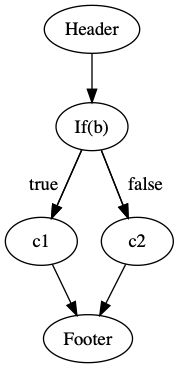
\includegraphics[scale=0.27]{ifElse}
\caption{If-Then-Else}
 \label{fig:ifElse}
\end{figure}
to the equivalent flattened program illustrated in Figure~\ref{fig:flatIfElse}.
\begin{figure}[hbt]
\centering
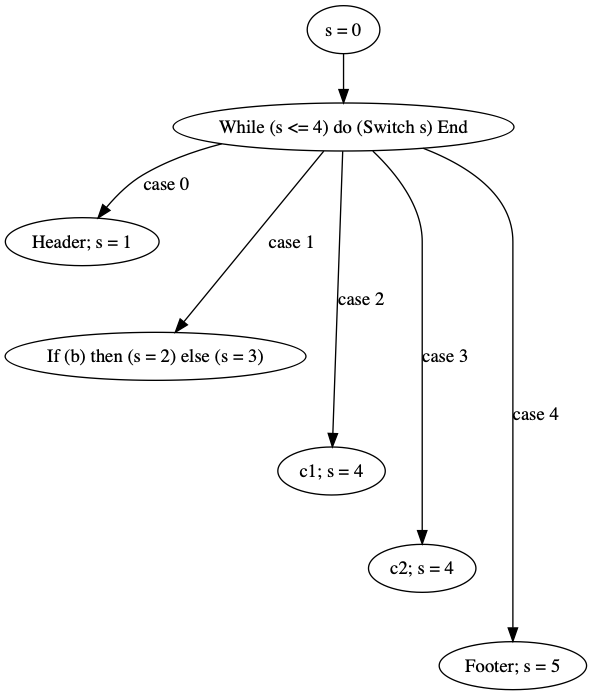
\includegraphics[scale=0.27]{ifElseFlat}
\caption{Flattened If-Then-Else}
 \label{fig:flatIfElse}
\end{figure}
%

In Section~\ref{4.4}, we briefly discuss other transformations that we have defined and proven correct but do not have space to provide details for.
For a thorough treatment of control flow flattening obfuscation and its effects in obstructing static analysis see \cite{Wang}. 

%\subsection{Flattening an If-Then-Else Construct}
%For the first half of this section, we will focus on a single transformation that turns an If-Then-Else construct into an equivalent flattened program (see listing \ref{lst:beforeflatten} which is adapted from \cite{Blazy2}):

%\begin{listing}
%\caption{If-Then-Else}
%\label{lst:beforeflatten}
%[
%frame=single,
%framesep=2mm,
%baselinestretch=1.2,
%fontsize=\footnotesize
%] {c}
%int i;
%i = 0; // Header
%if (i < 100) 
%{
%  i++;
%}
%else
%{
%  i = 9;
%}
%// Footer
%\end{minted}
%\end{listing}

%begin{listing}
%\caption{Flattened If-Then-Else}
%\label{lst:afterflatten}
%\begin{minted}
%[
%frame=single,
%framesep=2mm,
%baselinestretch=1.2,
%fontsize=\footnotesize
%] {c}
%int i;
%int swVar;
%swVar = 0;
%while (swVar <= 4) {
%  switch (swVar) {
%    case 0:
%      i = 0; // Header
%      swVar = 1;
%    case 1:
%      if (i < 100) {
%        swVar = 2;
%        break;
%      } else {
%        swVar = 3;
%        break;
%      }
%    case 2:
%      i++; swVar = 4;
%      break;
%    case 3:
%      i = 9; swVar = 4;
%      break;
%    case 4:
%      // Footer
%      swVar = 5;
%      break;
%  }
%}
%\end{minted}
%\end{listing}


%We will, in Section \ref{4.2}, first add the syntax and semantics\footnote{Phil: Do we need the syntax and semantics?  Amy: Thedefinition of \texttt{com} was originally left out entirely from IMP without Switch in the earlier sections, so it doesn't make sense to add it here.  In Section 2, I added a description and notation of \texttt{com}.  This section needs to be updated to do the same.} of Switch statements to the IMP language.  Then in Section \ref{4.3} we formalize the above transformation, define what it means for it to be correct, realize some additional conditions are required and formulate what those are, and then finally prove it so.


\subsection{Augmenting IMP with Switch (IMP+Switch)}\label{4.2}
%Before we can formalize control flow flattening of an If-Then-Else construct, we need to enrich IMP with the syntax and semantics of switch statements, which we'll call the \emph{IMP+Switch} language.  We'll also define a new type, $address$, which is just a wrapper for a $nat$ and a type $lc$ (list of commands) which is a list of possible switch branches indexed by $address$, and then redefine the type $com$ to support switch statements.
%
%\begin{verbatim}
%Definition address := nat.
%Definition lc := list (address * com).
%\end{verbatim}

%\begin{verbatim}
%Inductive com : Type :=
%  ...
%  | CSwitch : 
%    string -> 
%      list (address * com) -> com.
%\end{verbatim}

%Next, we create a function to search a $lc$ by address.
%\begin{verbatim}
%Fixpoint lc_lookup 
%  (tlc: lc) (adr: address): 
%     option com := ... 
%\end{verbatim}
%
%We'll also define a new type, $address$, which is just a wrapper for a $nat$ and a type $lc$ (list of commands) which is a list of possible switch branches indexed by $address$, and then redefine the type $com$ to support switch statements.
%
%We accordingly redefine the command evaluation semantics to include switch statements.
%
Before we can formalize control flow flattening of an If-Then-Else construct, we need to enrich IMP with the syntax and semantics of switch statements. We extend the original IMP language from~\cite{SFV2} and add the clause \texttt{| SWITCH v l} to the BNF grammar presented in Section~\ref{sec:syntaxsemantics}.  Here \texttt{v} is the name of the switch variable (which is $s$ in Figure~\ref{fig:flatIfElse}), represented as a Coq \texttt{string}.  The second argument \texttt{l} is a list of pairs (represented using Coq's built-in types for lists and pairs), where the first element of each pair is in $\mathbb{N}$, representing the case number in the switch statement, and the second element is a \texttt{com} representing the program associated with that number.
We accordingly redefine the command evaluation semantics (the definition of \verb|c / s1 \\ s2|) to include evaluation of switch statements.  In addition, we extend the proof in~\cite{SFV2} to show that evaluation is still deterministic with our new switch statements added to IMP.

%The following theorem and its proof already exist in \cite{SFV2}, but we must update it for our new formulation with switch statements.  The proof also introduces several new tactics and features which are worth explaining (see \cite{Weiyun} for details).\footnote{Phil: Are these ever explained below?  Amy: No, must be modified.}

%\begin{theorem}\label{deterministic}\index{deterministic}
%Command evaluation is deterministic, in the sense that if a command evaluates a state $st$ to a state $st1$, but %also to some (possibly) other state $st2$, then it must be the case that $st1 = st2$.  In Coq,
%\begin{verbatim}
%Theorem ceval_deterministic: 
%  forall c st st1 st2,
%   c / st \\ st1 -> 
%   c / st \\ st2 -> 
%         st1 = st2.
%\end{verbatim}
%\end{theorem}

\subsection{Flattening If-Then-Else in IMP+Switch}\label{flattenif}\label{4.3}

We wish to prove command equivalence between the original and transformed programs. We note that the switch variable $s$ is introduced in Figure~\ref{fig:flatIfElse} with value $0$ and ends with value $5$.  Hence, we need to preprocess the original program to be transformed by adding in these assignments.  We define two functions in Coq, one for preprocessing and one to transform the If-Then-Else statement into a switch statement.  
%We then prove that the two programs are equivalent using a new definition called \emph{evaluation invariance}.  
Both functions take a boolean condition, and two subprograms for the if-then and if-else branches.  They also take a header and footer, which are subprograms that are executed before and after the If-Then-Else statement, respectively.  These functions appear in Listings~\ref{listing:preprocess} and~\ref{listing:flatten}.
\begin{listing}
\caption{The \texttt{preprocess\_program} function}
\label{listing:preprocess}
\begin{minted}
[
frame=single,
framesep=2mm,
baselinestretch=1.2,
fontsize=\footnotesize
] {c}
Definition preprocess_program
  header cond c1 c2 footer : com :=
  swVar ::= 0 ;;
  header ;;
  IFB cond THEN c1 ELSE c2 FI ;;
  footer ;;
  swVar ::= 5.
\end{minted}
\end{listing}
%
\begin{listing}
\caption{The \texttt{transform\_program} function}
\label{listing:flatten}
\begin{minted}
[
frame=single,
framesep=2mm,
baselinestretch=1.2,
fontsize=\footnotesize
] {c}
Definition transform_program
  header cond c1 c2 footer : com :=
  swVar ::= 0 ;;
  WHILE (swVar <= 4) DO
    SWITCH swVar [
      (0, header ;; swVar ::= 1) ;
      (1, IFB cond THEN swVar ::= 2
          ELSE swVar ::= 3 FI) ;
      (2, c1 ;; swVar ::= 4) ;
      (3, c2 ;; swVar ::= 4) ;
      (4, footer ;; swVar ::= 5) ]
  END.
\end{minted}
\end{listing}
The difference is that the first function forms a regular If-Then-Else statement, and the second one forms the flattened version. From the components of the original program, it builds a switch statement wrapped in a while loop, with the cases appropriately handled.

%\begin{defin}
%We build an If-Then-Else statement to be flattened by the following function in Coq. The $header$ and %$footer$ parameters are simply any IMP commands that occur before and after, respectively, the %If-Then-Else statement. Since we wish to prove command equivalence between the original and transformed %programs, we note that $swVar$ is introduced with value $0$ and ends with value $5$ in the transformed %program; hence, we'll preprocess the original program to be transformed by adding in these assignments.
% 
%\begin{verbatim}
%Definition 
%  preprocess_program 
%    header cond c1 c2 footer: 
%      com := ... 
% \end{verbatim}
%\end{defin}
%
%\begin{defin}
%Transforming a program with control flow flattening on an If-Then-Else statement takes the If-Then-Else %components and builds a `switch' wrapped in a `while' with `cases' appropriately handled.
%\begin{verbatim}
%Definition 
%   transform_program 
%     header cond c1 c2 footer: 
%       com := ...
%\end{verbatim}
%\end{defin}

%\begin{defin}[WorldEater program]
%We'll use a minimal example program for this section, which we call \emph{WorldEater}, a %program that does nothing if the variable $X$ is zero, and assigns $X=1$ otherwise.

%\begin{verbatim}
%Definition WorldEater : com :=
%  IFB (X = 0) THEN
%    SKIP
%  ELSE
%    X ::= 1
%  FI.
%\end{verbatim}
%\end{defin}

%\begin{example}
%To preprocess $WorldEater$, we feed its components to \verb$preprocess_program$.
%\begin{verbatim}
%Definition PreprocessWorldEater := 
%  preprocess_program 
%    SKIP (X = 0) SKIP (X ::= 1) SKIP.
%\end{verbatim}

%Note that since the header and footer are mandatory, we add $SKIP$s, and the $swVar$ is set %to the same initial and final values so we can prove command equivalence to the transformed %program.
%\end{example}

%\begin{example}
%To transform $WorldEater$, we feed its components to $transform\_program$.
%\begin{verbatim}
%Definition TransWorldEater := 
%  transform_program 
%    SKIP (X = 0) SKIP (X ::= 1) SKIP.
%\end{verbatim}
%\end{example}

%\begin{example}\label{WE_example}
%The preprocessed and transformed $WorldEater$ programs are command equivalent.  In Coq,
%\begin{verbatim}
%Example WorldEaterTransEquiv : 
%  cequiv 
%    PreprocessWorldEater 
%    TransWorldEater.
%\end{verbatim}
%The proof (see \cite{Weiyun} for details) follows the same structure and ideas as the more %general Theorem \ref{maintheo} to come.
%\end{example}

Before we state the general theorem that any program's preprocessed and transformed forms are command equivalent, we have to fully account for the newly introduced switch variable which controls the switch statement, called \texttt{swVar} in Listings~\ref{listing:preprocess} and~\ref{listing:flatten}. If the original program already uses this variable in some way, then command equivalence will not necessarily hold. For example, suppose the header of the program to be transformed contains the assignment \texttt{swVar := 999}.  This would then completely bypass the entire flattened switch construct!  We avoid this problem with the definition below of \emph{evaluation invariance}, followed by a lemma about it.

\begin{defin}[Evaluation invariance]
A program \texttt{c} is \emph{evaluation invariant} with respect to a variable \texttt{X} if, for all states \texttt{st} and \texttt{st'} and all $\mathtt{n} \in \mathbb{N}$, \texttt{c} evaluates \texttt{st} to \texttt{st'} if and only if \texttt{c} evaluates \texttt{st} updated with \texttt{X --> n} to \texttt{st'} updated with \texttt{X --> n}.
In Coq:
\begin{verbatim}
Definition eval_invariant c X := 
  forall n st st',  c / st \\ st' <-> 
  c / st & { X --> n } 
      \\ st' & { X --> n }.
\end{verbatim}
\end{defin}
In other words, if the only thing that changes about the start state is the value of \texttt{X}, there is no impact on evaluation with the sole exception of the same change to \texttt{X} in the end state.  

\begin{lemma}\label{independence}
Evaluation invariance implies evaluation independence in the sense that, if a command \texttt{c} is evaluation invariant with respect to \texttt{X}, then if \texttt{c} evaluates a state \texttt{st} updated with \texttt{X -->  n} for some $\mathtt{n} \in \mathbb{N}$ to \texttt{st'}, then \texttt{c} also evaluates \texttt{st} to \texttt{st'}.  In Coq,
\begin{verbatim}
Lemma eval_inv_imp_eval_ind: 
  forall c X n st st', 
  eval_invariant c X ->
  c / st & { X --> n } \\ st' -> 
  c / st \\ st'.
\end{verbatim}
\end{lemma}

In order to state and prove the main theorem, we also need the related concept of \emph{boolean invariance}.
\begin{defin}[Boolean invariance]\index{boolean invariance}
A boolean expression \texttt{b} is \emph{boolean invariant} with respect to a variable \texttt{X} if for all states \texttt{st} and all $\mathtt{n} \in \mathbb{N}$, the boolean evaluation of \texttt{b} in \texttt{st} is the same as the boolean evaluation of \texttt{b} in \texttt{st} updated with \texttt{X --> n}.
In Coq:
\begin{verbatim}
Definition beval_invariant b X :=
  forall n st, beval st b = 
    beval (st & { X --> n }) b. 
\end{verbatim}
\end{defin}
%In other words, if the only thing that changes about the state in which boolean evaluation takes place is the value of $X$, then there is no impact on the evaluation.

We can now state the main theorem. In particular, control flow flattening of If-Then-Else constructs is sound in the following sense:
\begin{theorem}\label{maintheo}
Fix the variable \texttt{swVar} for the control flow flattening transformation.  
For any program of the form \verb$header;;IFB cond THEN c1 ELSE c2 END$ \verb$;; footer$, we have command equivalence between the following two programs (which we will call \texttt{p1} and \texttt{p2} in the proof below):
\begin{verbatim}
   preprocess_program header cond
                      c1 c2 footer
   transform_program header cond
                      c1 c2 footer
\end{verbatim}

as long as the following hold:
\begin{itemize}
    \item The commands \texttt{footer}, \texttt{c1}, and \texttt{c2} are evaluation invariant with respect to \texttt{swVar}.
    \item The boolean condition \texttt{cond} is boolean invariant with respect to \texttt{swVar}.
\end{itemize}
In Coq:
\begin{verbatim}
Theorem AllTransEquiv:
  forall header cond c1 c2 footer, 
  eval_invariant c1 swVar -> 
  eval_invariant c2 swVar -> 
  eval_invariant footer swVar ->
  beval_invariant cond swVar ->
  cequiv (preprocess_program header
                  cond c1 c2 footer) 
         (transform_program header
                  cond c1 c2 footer).
\end{verbatim}
\end{theorem}
\emph{Proof Sketch.}
Proving command equivalence in this case requires proving that for all states \texttt{st} and \texttt{st'}, both \verb|p1 / st \\ st' -> p2 / st \\ st'| and \verb|p2 / st \\ st' -> p1 / st \\ st'|.  Each case has two subcases depending on whether \texttt{cond} is true or false.  We discuss only the first case, with the subcase where \texttt{cond} is true.  In the Coq proof, we work in the backward direction, starting with the statement of the theorem and breaking it down into subgoals step-by-step by applying tactics.  After numerous steps, the subcase of interest is expressed as the Coq goal in Figure~\ref{comequiproof}.

%\begin{listing}
%\caption{The \texttt{transform\_program} function}
%\label{listing:proof}
%\begin{minted}
%[
%frame=single,
%framesep=2mm,
%baselinestretch=1.2,
%fontsize=\footnotesize,
%escapeinside=??
%] {c}
\begin{figure}
\begin{verbatim}
  cond : bexp
  header, c1, c2, footer : com
  st, st', s0, s1, s2, s3 : state
  HI1 : eval_invariant c1 swVar
  HI2 : eval_invariant c2 swVar
  HIf : eval_invariant footer swVar
  HB : beval_invariant cond swVar
  H2 : (swVar ::= 0) / st \\ s0
  H3 : header / s0 \\ s1
  H4 : 
    (IFB cond THEN c1 ELSE c2 FI) 
    / s1 \\ s2
  H6 : footer / s2 \\ s3
  H11 : (swVar ::= 5) / s3 \\ st'
  A0 : aeval s0 swVar = 0
  A5 : aeval st' swVar = 5
  Hcond : beval s1 cond = true
  ============================
  (swVar ::= 0;;
   WHILE swVar <= 4
   DO SWITCH swVar
      [(0, header;; swVar ::= 1);
       (1, IFB cond THEN swVar ::= 2 
           ELSE swVar ::= 3 FI);
       (2, c1;; swVar ::= 4);
       (3, c2;; swVar ::= 4);
       (4, footer;; swVar ::= 5)]
   END) / st \\ st'
\end{verbatim}
\caption{Command equivalence proof step}
    \label{comequiproof}
\end{figure}

The formulas above the double line are the current hypotheses, while the statement to be proven is below the line. Many of the hypotheses come from breaking down the program \texttt{p1} into evaluation steps for single statements. They come from the definition of the evaluation relation, which as discussed, defines the operational semantics of IMP+Switch.  For example, \texttt{H2} expresses that the assignment statement \texttt{swVar ::= 0} is evaluated in the start state \texttt{st} resulting in the intermediate state \texttt{s0}, while \texttt{H3} expresses that evaluating the header starting from the intermediate state \texttt{s0} results in a new intermediate state \texttt{s1}.  The last 3 hypotheses state some facts about the values of \texttt{swVar} in the start and end states and show the value of \texttt{cond} for this subcase. To prove the conclusion, the definition of evaluation is again important, along with the fact that the evaluation relation is deterministic.


\subsection{Transforming a While-Do-End Construct}\label{4.4}
We now switch gears and briefly discuss \emph{dismantling} and then \emph{flattening} a While-Do-End construct, focusing on an example described in \cite{Wang}.
For this particular transformation, we start with a program with a While-Do-End construct, and dismantle it into a number of basic blocks (where each block is a sequence of non-control flow commands ending with a control flow command), essentially replacing the While-Do-End construct with conditional GoTo statements at the end of some blocks.  During execution, the targets of these GoTos are determined dynamically with conditions on some variable in memory, instead of a direct (constant) address as the jump target. Following \cite{Wang} we call this intermediate transformation a dismantling.
Dismantling is then followed by a flattening operation, reminiscent of the flattening transformation above.
%In keeping consistent with prior terminology, this transformation will be called flattening.  We'll develop a different language in the next section, however, and model this a bit differently from the switch statements of Sections \ref{4.2} and \ref{4.3}, as we need to consider basic blocks as first class citizens.

%\subsection{Wrapping IMP in a Flowchart Language (IMP+Flow)}\index{IMP+Flow}

%In this section,\footnote{AF: Address Phil's comments about flowchart languages, maybe by adding a reference to the Software Foundations book, where it is used there.} we describe a new lower-level formal language which will be used to represent the example from the previous section.  We'll call this language \emph{IMP+Flow}, short for flowchart\footnote{Note that our formulation for \emph{flowchart} is different from \cite{SFV2}}. We also define evaluation relations for basic blocks and programs of basic blocks (see \cite{Weiyun} for details).

%This language is similar to intermediate languages that are transpiled to and used in the commercial obfuscation tools such as Cloakware's obfuscation engine \cite{Cloakware}. While very cumbersome to actually write programs in, it is well-suited to control flow related algorithms due to its treatment of basic blocks (of code) as first-class citizens.

%Note here that the underlying program is the original IMP, and not the IMP+Switch defined in Section \ref{4.2}.  We handle switch statements differently here, by defining them as a type of block.

For this transformation, we modify IMP once again.  This time, we replace the switch command of the previous section with a lower-level language (which we call IMP+Flow since it explicitly deals with flow of control constructs like jumps) containing basic blocks, with a switch statement as one of the kinds of blocks.
This language is similar to intermediate languages into which higher-level programs are transpiled, and which are used in commercial obfuscation tools such as Cloakware's obfuscation engine \cite{Cloakware}.

In Coq, we introduce a new type called \texttt{comBlock}, which encodes the following grammar: 
\texttt{bJump c l | bCond c b l l | bSwitch c v m | bEnd c}. 
Each kind of block consists of a command together with an instruction of how to find the next block.
They include 1) an unconditional jump where the next block is denoted by a label \texttt{l} represented as a Coq string, 2) a conditional jump, where \texttt{b} is a \texttt{bexp} and the two labels indicate where to jump in the true and false cases, 3) a switch command, with switch variable \texttt{v} and mapping \texttt{m}, which maps values of the switch variable to labels, and 4) a terminal block.  A program is then a pair consisting of an initial command block and a \emph{block dictionary}, which maps labels to command blocks.  We must also extend the definition of the evaluation relation to command blocks.  (We omit the details. As usual, see \cite{Weiyun,WeiRepo}.)

%\subsection{Flattening While-Do-End in IMP+Flow}

We illustrate this notion of dismantling and flattening with the example mentioned earlier.  The original program is a single block containing the IMP program below:
\begin{verbatim}
  WHILE (A <= 2) DO
    B ::= A + B ;;
    IFB (!(B <= 4)) THEN
      B ::= B - 1
    ELSE SKIP FI ;;
    A ::= A + 1
  END ;;
  RETURN ::= A * B.
\end{verbatim}
We do not describe the transformation any further, but just note that the transformed program contains the following blocks, and execution starts at block \texttt{L1}.
\begin{verbatim}
"L1" --> bConditional SKIP
         (! (A <= 2)) "L4" "L3";
"L2" --> bJump (A ::= A + 1) "L1";
"L3" --> bConditional (B ::= A + B)
         (B <= 4) "L2" "L5";
"L4" --> bEnd (RETURN ::= A * B); 
"L5" --> bJump (B ::= B - 1) "L2"
\end{verbatim}
 %We transform\footnote{Phil:Too compressed.  Maybe put the details into an appendix.} it into the dismantled version which is basically the same program but using basic blocks and labels and jumps. We show that the `DismantledProgram` will, like the `OriginalProgram`, evaluate a state that begins with $A = 1$ and $B = 2$ to a final state that has $RETURN = 12$. We then manually build the flattened version of `DismantledProgram` component by component and show that the resulting `FlattenedProgram` will, like the `OriginalProgram` and the `DismantledProgram` evaluate a state that begins with $A = 1$ and $B = 2$ to a final state that has $RETURN = 12$ (see \cite{Weiyun} for details).
We have proved that both versions of the program, when starting in a state with \texttt{A = 1} and \texttt{B = 2}, evaluate to the same final state with \texttt{RETURN = 12}. Future work includes extending our command equivalence theorem to this kind of transformation.

\section{Obfuscation in Coq: Related Work}
%There have been three papers, in all of which Sandrine Blazy (Universit\'{e} de Rennes 1) appears as a coauthor, that study code obfuscation in Coq.
There have been three papers by Sandrine Blazy and co-authors that study code obfuscation in Coq, which we discuss here.

%\subsection*{Towards a formally verified obfuscating compiler}
The first paper
%, \emph{Towards a formally verified obfuscating compiler} 
\cite{Blazy1} also uses IMP (their own formulation and not the one from \cite{SFV2}) as the language for obfuscation, but studies data and layout obfuscation techniques, as opposed to the control obfuscation techniques which opaque predicates and control flow flattening fall under \cite{CollbergTax}.
%
%The first particular transformation studied herein is obfuscating integer constants, wherein all integer values are substituted by different ones in a distorted semantics using an obfuscating function $O: \mathbb{N} \to \mathbb{N}$.  The other discussed is variable encoding, which changes the names of variables.  A real-life application of this could be, for instance, to change a descriptive variable name like $account\_balance$ to a string of gibberish.
%
They first consider obfuscating integer constants using a function that maps each integer to a different one, and then performing a substitution using this mapping.  They also consider changing variable names, which can be used, for example, to change a descriptive variable name like $account\_balance$ to a string of gibberish.
%This is an inherently different class of techniques from the ones studied in the present work, and one can make a simple combinatorial argument that putting them together in the same obfuscation transformation would generate a synergistic effect on making a program more difficult to analyze.
Such techniques are inherently different from the ones we have studied. One can make a simple combinatorial argument that putting them together in the same obfuscation transformation would generate a synergistic effect, making a program possibly much more difficult to analyze.

%\subsection*{Formal verification of control-flow graph flattening}
The second paper
%, \emph{Formal verification of control-flow graph flattening} 
\cite{Blazy2} also studies control flow flattening, but the authors use the Clight language of CompCert \cite{CompCert} (the formally verified C compiler in Coq) and prove the correctness of the obfuscation in that setting, from which the correctness of the compilation process follows ``for free'' from CompCert's own proofs of semantic preservation.

On the one hand, the approach in \cite{Blazy2} is less elementary and less accessible, as it works with a nontrivial subset of the real C language, but on the other it is clear evidence that formal verification of obfuscation techniques need not be restricted to a small language like IMP. Other real-world practicalities considered in \cite{Blazy2} include simulation techniques and analysis of running time.

The work in \cite{Blazy2} also discusses some solutions for improving the stealth of control flow flattening, such as splitting a switching variable into two different variables that are updated at different points of a program, as well as randomly encoding the values of the switch cases so they don't just correspond to consecutive numbers.  %These are necessary considerations, since we need to think one level higher about attackers, and obfuscate the fact that we are obfuscating particular parts of our code with control-flow graph flattening in the first place!

In comparing the work in \cite{Blazy2} to ours, we believe there is merit both in the IMP and the CompCert routes.  In the former, the language used is of minimal complexity, which allows not only for specifications and proofs of transformations to be developed quicker without being bogged down in unnecessarily complicated features of the underlying language, but is also better suited for pedagogical purposes (see our research goal \ref{goal2}). IMP is also Turing complete, so from a theoretical point of view there is no loss of generality in proofs made using it---they can always be adapted to CompCert later.  On the other hand, CompCert is, of course, closer to languages that would be of interest to real-world applications and so more practical in that sense.

The authors of \cite{Blazy2} also 
%ran into a similar issue as we did; they 
needed to separate switching variables from those in the program to be transformed (as we did), but their solution was different. They instead use a function to parse the program to be transformed and generate a fresh variable which doesn't appear there to be used for the transformation.  From a practical point of view, this approach is perhaps more natural, and in line with how a real obfuscating tool would function---generating new variables rather than demand that a certain specifically named variable doesn't exist in the source program.  Theoretically, though, these are equivalent, since any program can contain only finitely many variable names, and there are an infinite number to choose from.

%\subsection*{Formal verification of a program obfuscation based on mixed boolean-arithmetic expressions}
The third paper
%, \emph{Formal verification of a program obfuscation based on mixed boolean-arithmetic expressions}
\cite{Blazy3} continues to work in Clight, and studies obfuscations that involve mixing arithmetic operators and bitwise boolean operators.  This is another data obfuscation that appears frequently in real-world binary code, but as it is based on features wildly beyond the capabilities of IMP, a detailed discussion is beyond the scope of the present work.

\section{Future Work}
The work done to date on formal verification of obfuscation, both in the present work and in the papers of Blazy et al., while providing a solid proof-of-concept that obfuscation tools of the future could support formal verification, are still limited in scope in the sense that they treat individual transformations.

A real world obfuscator mixes many different transformations together at once, often in non-deterministic ways for \emph{diversification} of obfuscations, and so some form of compositionality would need to be implemented on these formal proofs to be able to use them together and preserve the desired formulation of correctness. 

%Earlier (contribution item \ref{itm:1}) we mentioned how our obfuscators would generate additional assertions to show the obfuscated program preserves a desired behaviour of the original program. While we have worked out offline proofs for certain obfuscations, such as certain opaque predicates, we still need a way to integrate these proofs in the machinery of ``decorated programs'' that \emph{IMP} already provides. 
Earlier (first contribution item) we mentioned how our obfuscators would generate additional assertions to show the obfuscated program preserves a desired behaviour of the original program. While we have worked out offline proofs for certain obfuscations, such as some new opaque predicates, we still need a way to integrate these proofs into the machinery of ``decorated programs'' that IMP already provides. 

%(along with the three aforementioned pieces of related work)
Furthermore, we (along with the work of Blazy et al.)
have, in the formal setting of Coq, only tackled one desired property of obfuscation---correctness.  That is, some form of the semantics of the program, or relationship between inputs and outputs, should be preserved (obfuscation property \ref{itm:firstproperty} mentioned in the introduction, i.e, the functionality property). But there are, of course, other properties that have not been touched upon, namely properties \ref{itm:secondproperty} and \ref{itm:thirdproperty}.

In closing, we stress, once more, that it \emph{is} important to actually apply formal specifications and methods to security goals and metrics in some form, so we can come full circle and give prospective clients of an obfuscation tool a clear answer to the \emph{other} big question ``How exactly will using this improve the security of my programs?" and be able to back our answer with a proof that it actually does so.

%\begin{thebibliography}{10}
\providecommand{\url}[1]{#1}
\csname url@samestyle\endcsname
\providecommand{\newblock}{\relax}
\providecommand{\bibinfo}[2]{#2}
\providecommand{\BIBentrySTDinterwordspacing}{\spaceskip=0pt\relax}
\providecommand{\BIBentryALTinterwordstretchfactor}{4}
\providecommand{\BIBentryALTinterwordspacing}{\spaceskip=\fontdimen2\font plus
\BIBentryALTinterwordstretchfactor\fontdimen3\font minus
  \fontdimen4\font\relax}
\providecommand{\BIBforeignlanguage}[2]{{%
\expandafter\ifx\csname l@#1\endcsname\relax
\typeout{** WARNING: IEEEtran.bst: No hyphenation pattern has been}%
\typeout{** loaded for the language `#1'. Using the pattern for}%
\typeout{** the default language instead.}%
\else
\language=\csname l@#1\endcsname
\fi
#2}}
\providecommand{\BIBdecl}{\relax}
\BIBdecl

\bibitem{Floyd}
R.~W. Floyd, ``Assigning meanings to programs,'' in \emph{Program
  Verification}.\hskip 1em plus 0.5em minus 0.4em\relax Springer, 1993, pp.
  65--81.

\bibitem{Hoare}
C.~A.~R. Hoare, ``An axiomatic basis for computer programming,''
  \emph{Communications of the ACM}, vol.~12, no.~10, pp. 576--580, 1969.

\bibitem{Eiffel}
B.~Meyer, ``Applying'design by contract','' \emph{Computer}, vol.~25, no.~10,
  pp. 40--51, 1992.

\bibitem{b7}
G.~C. Necula, ``Proof-carrying code,'' in \emph{Proceedings of the 24th ACM
  SIGPLAN-SIGACT symposium on Principles of programming languages}, 1997, pp.
  106--119.

\bibitem{CompCert}
X.~Leroy, ``Formal verification of a realistic compiler,'' \emph{Communications
  of the ACM}, vol.~52, no.~7, pp. 107--115, 2009.

\bibitem{BanescuCGNP16}
S.~Banescu, C.~Collberg, V.~Ganesh, Z.~Newsham, and A.~Pretschner, ``Code
  obfuscation against symbolic execution attacks,'' in \emph{Proceedings of the
  32nd Annual Conference on Computer Security Applications}, 2016, pp.
  189--200.

\bibitem{Coq}
B.~Barras, S.~Boutin, C.~Cornes, J.~Courant, J.-C. Filliatre, E.~Gimenez,
  H.~Herbelin, G.~Huet, C.~Munoz, C.~Murthy \emph{et~al.}, ``The coq proof
  assistant reference manual: Version 6.1,'' 1997.

\bibitem{SFV2}
B.~C. Pierce, A.~A. de~Amorim, C.~Casinghino, M.~Gaboardi, M.~Greenberg,
  C.~Hricu, V.~Sj{\"o}berg, A.~Tolmach, and B.~Yorgey, ``Programming language
  foundations, volume 2 of software foundations,'' 2010.

\bibitem{Blazy2}
S.~Blazy and A.~Trieu, ``Formal verification of control-flow graph
  flattening,'' in \emph{Proceedings of the 5th ACM SIGPLAN Conference on
  Certified Programs and Proofs}, 2016, pp. 176--187.

\bibitem{Weiyun}
W.~Lu, ``Formally verified code obfuscation in the coq proof assistant,'' Ph.D.
  dissertation, Universit{\'e} d'Ottawa/University of Ottawa, 2019.

\bibitem{WeiRepo}
\BIBentryALTinterwordspacing
W.~L{u}, ``Github repository to accompany the present research,'' 2019.
  [Online]. Available:
  \url{https://github.com/weiyunlu/coq-certified-obfuscation}
\BIBentrySTDinterwordspacing

\bibitem{CoNa}
J.~Nagra and C.~Collberg, \emph{Surreptitious Software: Obfuscation,
  Watermarking, and Tamperproofing for Software Protection: Obfuscation,
  Watermarking, and Tamperproofing for Software Protection}.\hskip 1em plus
  0.5em minus 0.4em\relax Pearson Education, 2009.

\bibitem{Prada}
M.~Dalla~Preda, M.~Madou, K.~De~Bosschere, and R.~Giacobazzi, ``Opaque
  predicates detection by abstract interpretation,'' in \emph{International
  Conference on Algebraic Methodology and Software Technology}.\hskip 1em plus
  0.5em minus 0.4em\relax Springer, 2006, pp. 81--95.

\bibitem{Wang}
C.~Wang, J.~Hill, J.~Knight, and J.~Davidson, ``Software tamper resistance:
  Obstructing static analysis of programs,'' Technical Report CS-2000-12,
  University of Virginia, 12 2000, Tech. Rep., 2000.

\bibitem{Cloakware}
C.~Liem, Y.~X. Gu, and H.~Johnson, ``A compiler-based infrastructure for
  software-protection,'' in \emph{Proceedings of the third ACM SIGPLAN workshop
  on Programming languages and analysis for security}, 2008, pp. 33--44.

\bibitem{Blazy1}
S.~Blazy and R.~Giacobazzi, ``Towards a formally verified obfuscating
  compiler,'' 2012.

\bibitem{CollbergTax}
C.~Collberg, C.~Thomborson, and D.~Low, ``A taxonomy of obfuscating
  transformations,'' 1997.

\bibitem{Blazy3}
S.~Blazy and R.~Hutin, ``Formal verification of a program obfuscation based on
  mixed boolean-arithmetic expressions,'' in \emph{Proceedings of the 8th ACM
  SIGPLAN International Conference on Certified Programs and Proofs}, 2019, pp.
  196--208.

\end{thebibliography}

\bibliographystyle{IEEEtranS}
\bibliography{eurosp-2020-template}
\end{document}
